\chapter{Running OpenDQ}
\label{sec:04-running}
This section explains how to obtain the OpenDQ project from GitHub and how to load, execute and debug it on the OpenMote platform. The section assumes that the user has the appropriate hardware and has setup a working environment, as described in Section~\ref{sec:02-hardware} and Section~\ref{sec:03-installing} respectively. If that is not the case, please refer to such sections prior to following this section.

%%
% Hardware requirements
%%
\section{Hardware requirements}
In order to run and debug the OpenDQ software a minimum of hardware is required. At a minimum, two OpenMote-CC2538, one OpenBase and one OpenBattery are required. Such hardware can be bought as an OpenBronze kit, as depicted in Figure~\ref{fig:openbronze}, from the OpenMote website. However, a OpenGold kit is required in order to be able to demonstrate all the characteristics of the OpenDQ implementation.

% OpenBronze kit
\begin{figure}[!it]
    \centering
	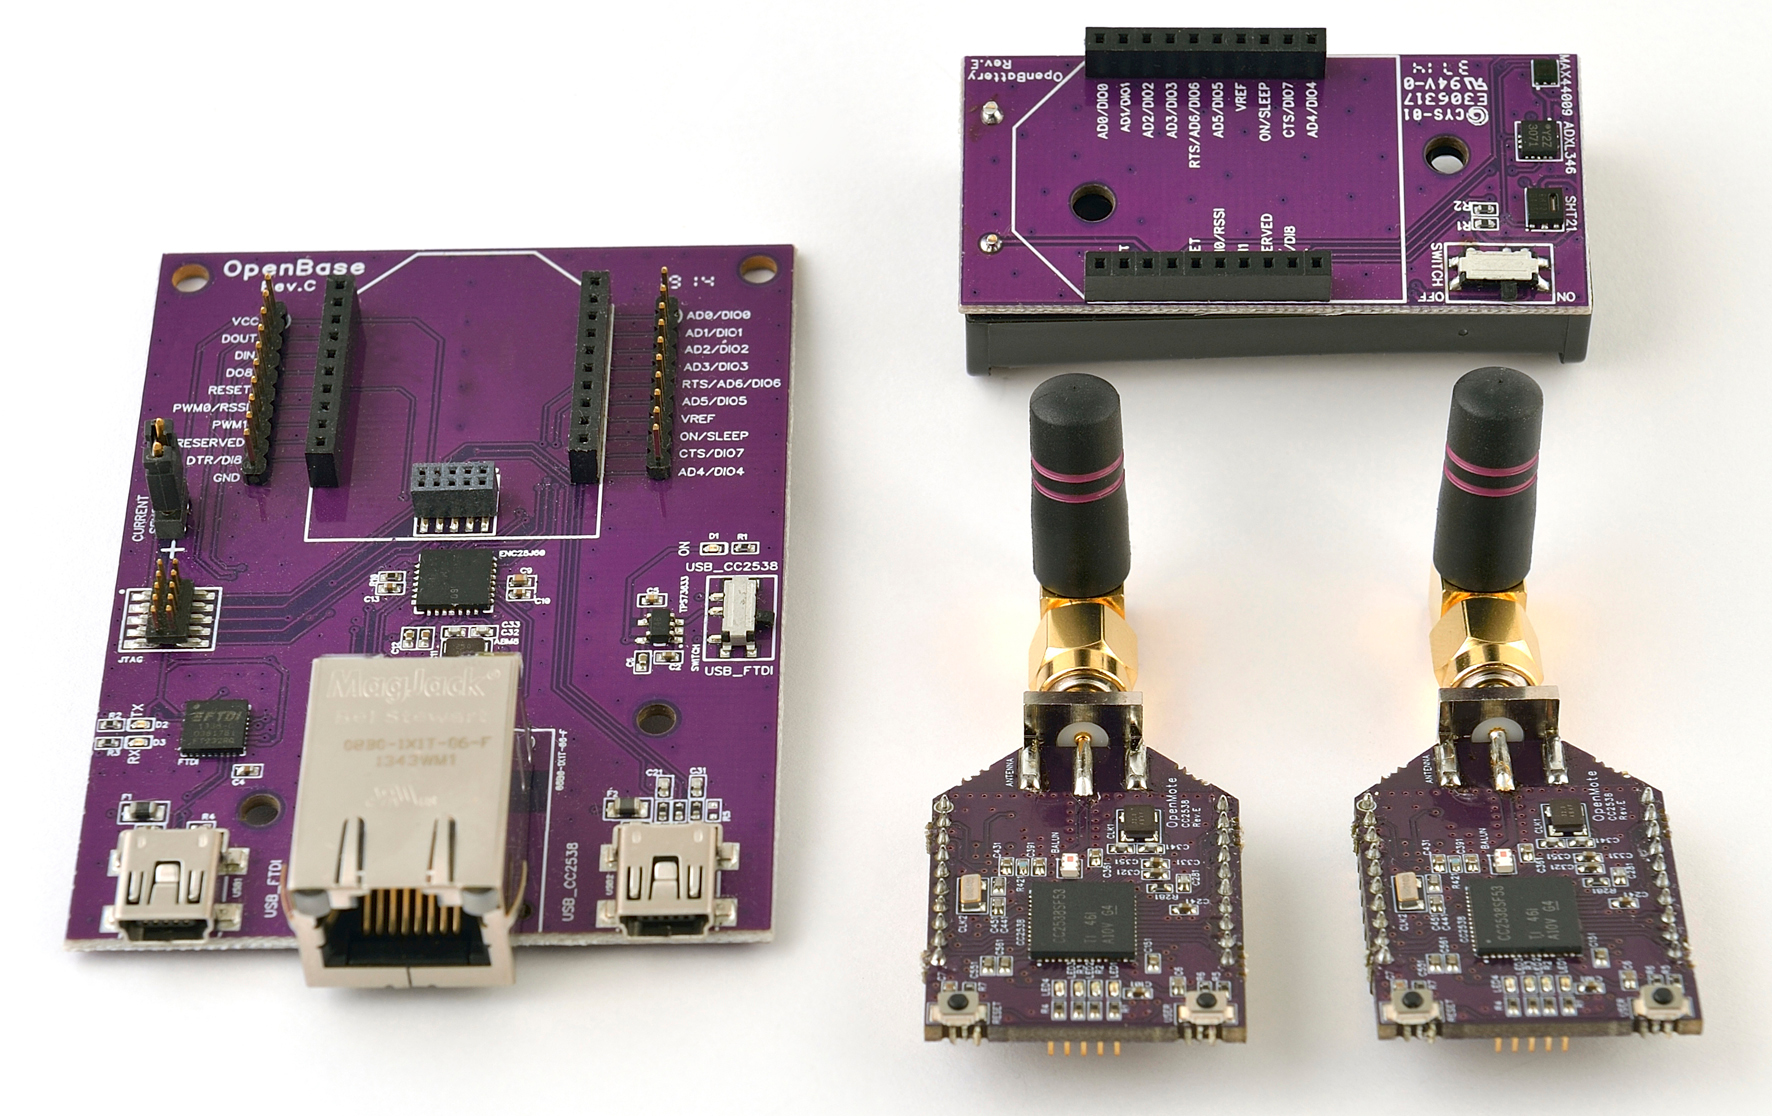
\includegraphics[width=0.75\linewidth]{01-bronzekit}
    \caption{Contents of an OpenBronze kit.}
    \label{fig:openbronze}
\end{figure}

In addition to OpenBronze kit, the following hardware is required in order to run and debug the OpenDQ project:
\begin{itemize}
\item Segger J-Link EDU. Required to load and debug the OpenDQ project on the OpenMote-CC2538 hardware.
\item ARM 20-to-10 pin adapter. Required to connect the Segger J-Link EDU to the OpenBase.
\item USB mini cable. Required to power the OpenBase board.
\item 2xAAA batteries. Required to power the OpenBattery board.
\end{itemize}

%%
% Obtain the OpenDQ project
%%
\section{Obtain the OpenDQ project}
The OpenDQ project is stored in GitHub (https://github.com). In order to obtain the OpenDQ project from GitHub navigate to the folder where you want the software to be installed. In this documentation it is assumed that the OpenDQ resides in a folder named OpenDQ in the user home folder. To clone the OpenDQ project from GitHub issue the following commands on a terminal window.

\begin{verbatim}
cd ~
git clone http://github.com/OpenMote/OpenDQ ~/OpenDQ
\end{verbatim}

If the process is successful the OpenDQ project will be in your home folder and a screen similar to Figure~\ref{fig:06-clone} should be displayed. Also, a folder with the contents displayed in Figure~\ref{fig:06-folder} should be created in the user home folder.

% Cloning the OpenDQ project from GitHub.
\begin{figure}[!ht]
    \centering
	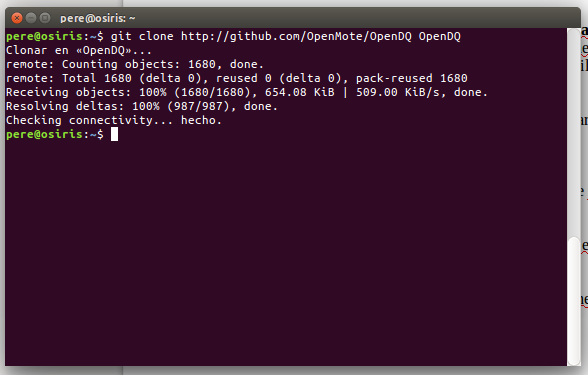
\includegraphics[width=0.75\linewidth]{06-clone}
    \caption{Cloning the OpenDQ project from GitHub.}
    \label{fig:06-clone}
\end{figure}

% Main folder structure of the OpenDQ distribution
\begin{figure}[!ht]
    \centering
	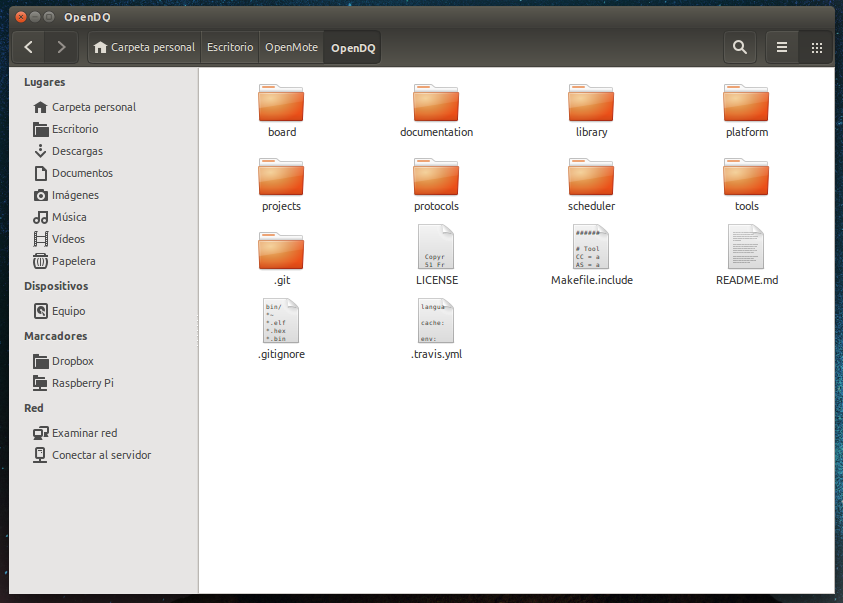
\includegraphics[width=0.75\linewidth]{06-folder}
    \caption{Main folder structure of the OpenDQ distribution.}
    \label{fig:06-folder}
\end{figure}

%%
% Compiling CC2538 firmware library
%%
\section{Generate the Texas Instruments CC2538 firmware library}
Once the OpenDQ project source code has been obtain, the next step is to create the statically linked library that contains the firmware for the Texas Instruments CC2538 SoC. This step is required because the OpenDQ project has file names that collide with those of the Texas Instruments CC2538 firmware library. In order to compile the Texas Instruments CC2538 firmware library navigate to the appropriate directory and execute the $libcc2538_setup.py$ Python script using the following commands.

\begin{verbatim}
cd ~/OpenDQ/platform/cc2538/library
python libcc2538_setup.py
\end{verbatim}

If the process is successful the Texas Instruments CC2538 firmware library will be automatically generated and copied to the appropriate directory and a screen similar to Figure~\ref{fig:libcc2538} should be displayed. To check if the Texas Instruments CC2538 firmware library has been correctly installed, check that a file named $libcc2538.a$ has been created in the $~/OpenDQ/platform/cc2538$ directory.

% Generating the libcc2538 library
\begin{figure}[!t]
    \centering
	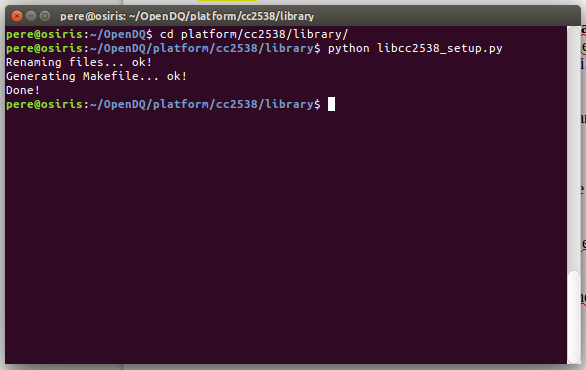
\includegraphics[width=0.75\linewidth]{06-libcc2538}
    \caption{Generating the libcc2538 library.}
    \label{fig:libcc2538}
\end{figure}

%%
% Compiling Node/Gateway projects
%%
\label{sec:06-firmware}
\section{Compile, load and debug the Node/Gateway projects}
Once the Texas Instruments CC2538 firmware library ($libcc2538.a$) has been generated it is possible to compile the Node and Gateway projects. The mechanism to compile, load and debug the Node and Gateway firmware projects to the OpenMote-CC2538 board is based on a Makefile system that is deployed across all the project folder structure. Such mechanism does not need to be modified by the user unless new files need to be compiled.

The following steps assumes that an OpenMote-CC2538 is connected to an OpenBase which, in turn, is connected to a computer via a USB port (using the USB\_FTDI port), as depicted in Figure~\ref{fig:06-openbase}. Please notice that the blue cable that connects the GND pin with the ON/SLEEP pin on the OpenBase are required to ensure that the OpenMote-CC2538 enters the bootload mode when the reset button is pressed. When the bootload mode is entered the 4 LEDs on the OpenMote-CC2538 become dim.

% Connecting an OpenMote-CC2538 to a computer with an OpenBase.
\begin{figure}[!ht]
    \centering
	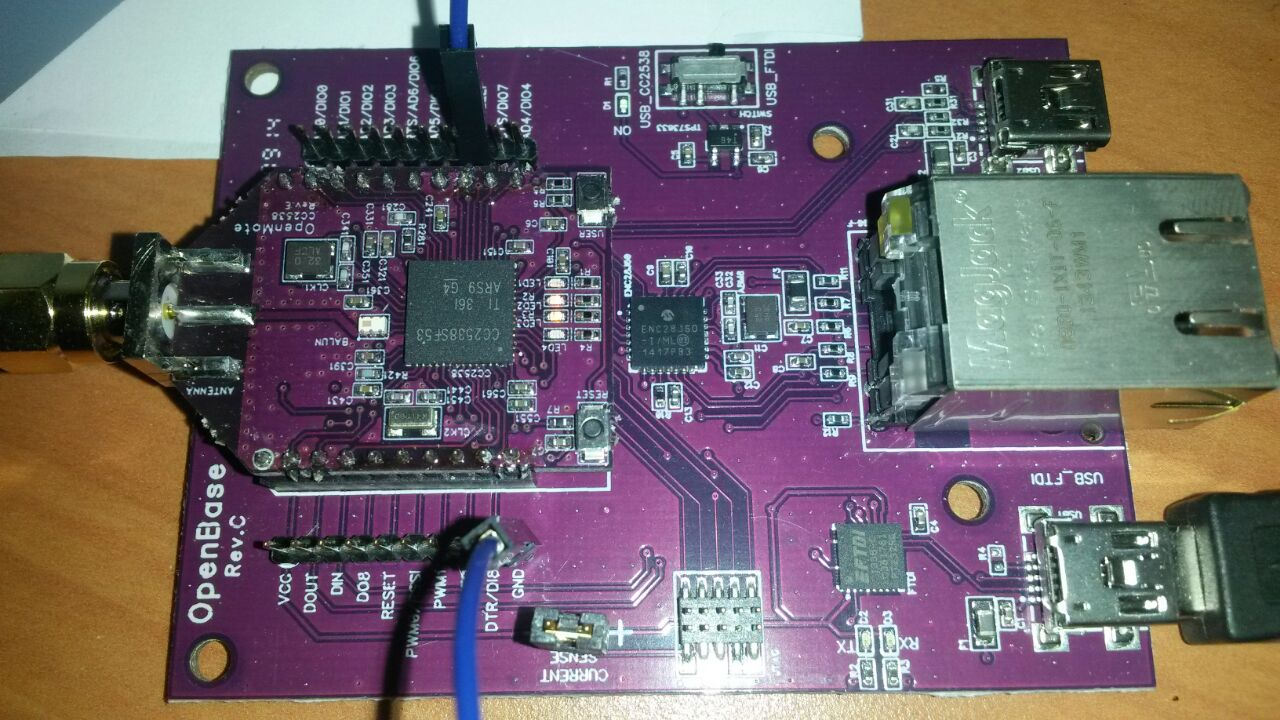
\includegraphics[width=0.75\linewidth]{06-openbase}
    \caption{Connecting an OpenMote-CC2538 to a computer with an OpenBase.}
    \label{fig:06-openbase}
\end{figure}

In order to compile, load and debug the Node or Gateway firmware projects navigate to the appropriate directory. For the Node project go to $~/OpenDQ/projects/Node/src$. For the Gateway project go to $~/OpenDQ/projects/Gateway/src$.

In order to compile the Node/Gateway project using the Makefile system execute the following command. If the process is successful, a screen similar to Figure~\ref{fig:06-compile} should be displayed.

\begin{verbatim}
make TARGET=cc2538 all
\end{verbatim}

% Compiling the Node/Gateway project
\begin{figure}[!ht]
    \centering
	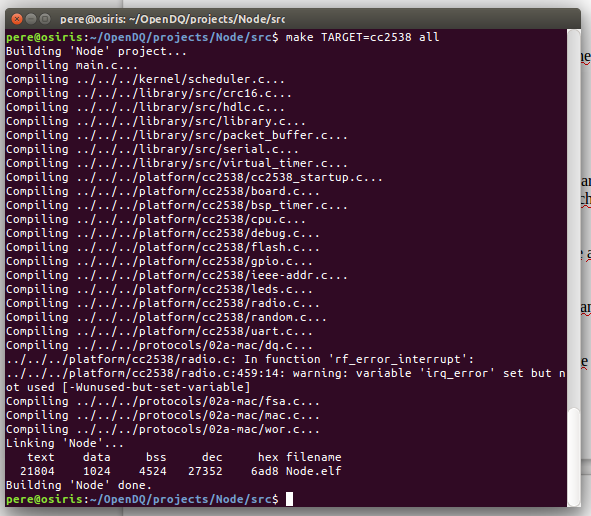
\includegraphics[width=0.75\linewidth]{06-compile}
    \caption{Compiling the Node/Gateway project.}
    \label{fig:06-compile}
\end{figure}

Once the Node/Gateway project has been build using the Makefile system a folder (bin) and three new files containing various versions of the firmware image (elf, hex and bin) will be created, as displayed in Figure~\ref{fig:06-binaries}. It is possible to clean the project compilation by issuing the following command. After that, the folder and the firmware images will be removed.

\begin{verbatim}
make TARGET=cc2538 clean
\end{verbatim}

% Folder containing the binaries for the Node project.
\begin{figure}[!ht]
    \centering
	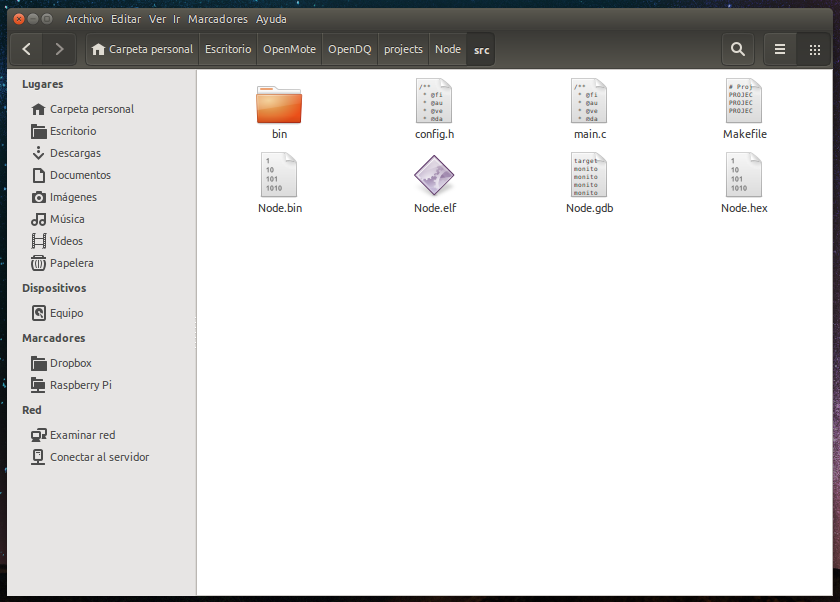
\includegraphics[width=0.75\linewidth]{06-binaries}
    \caption{Folder containing the binaries for the Node project.}
    \label{fig:06-binaries}
\end{figure}

Once the Node/Gateway project has been build, there are two mechanism strategies to load the generated firmware image to the OpenMote-CC2538. The first mechanism is based on the CC2538 bootloader and uses the serial port on the OpenBase. The second mechanism is based on the JTAG and uses that JTAG port on the OpenBase. Both mechanisms are described next.

To load the firmware to the OpenMote-CC2538 using the bootloader mechanism execute the following command. Such command assumes that the OpenMote-CC2538 is in bootloader mode. If the execution is successful a screen similar to Figure~\ref{fig:06-bsl} should appear. After that the OpenMote-CC2538 will start blinking the green LED periodically.

\begin{verbatim}
make TARGET=cc2538 bsl
\end{verbatim}

% Loading the Node/Gateway firwmare using the OpenMote-CC2538 bootloader.
\begin{figure}[!ht]
    \centering
	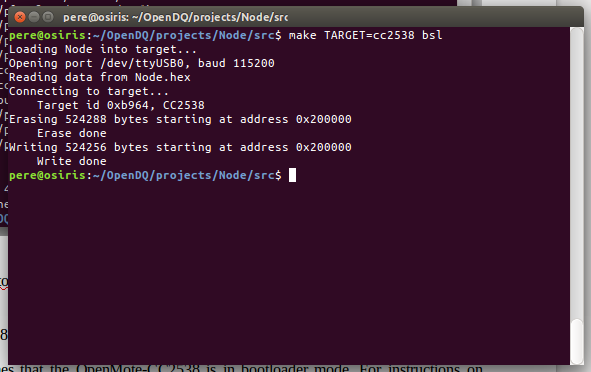
\includegraphics[width=0.75\linewidth]{06-bsl}
    \caption{Loading the Node/Gateway firwmare using the OpenMote-CC2538 bootloader.}
    \label{fig:06-bsl}
\end{figure}

To use the JTAG to load the Node/Gateway firmware image to the OpenMote-CC2538, first connect the Segger J-Link EDU probe to the OpenBase as depicted in Figure~\ref{fig:06-jtag}.

% Connecting the Segger J-Link probe to the OpenBase
\begin{figure}[!ht]
    \centering
	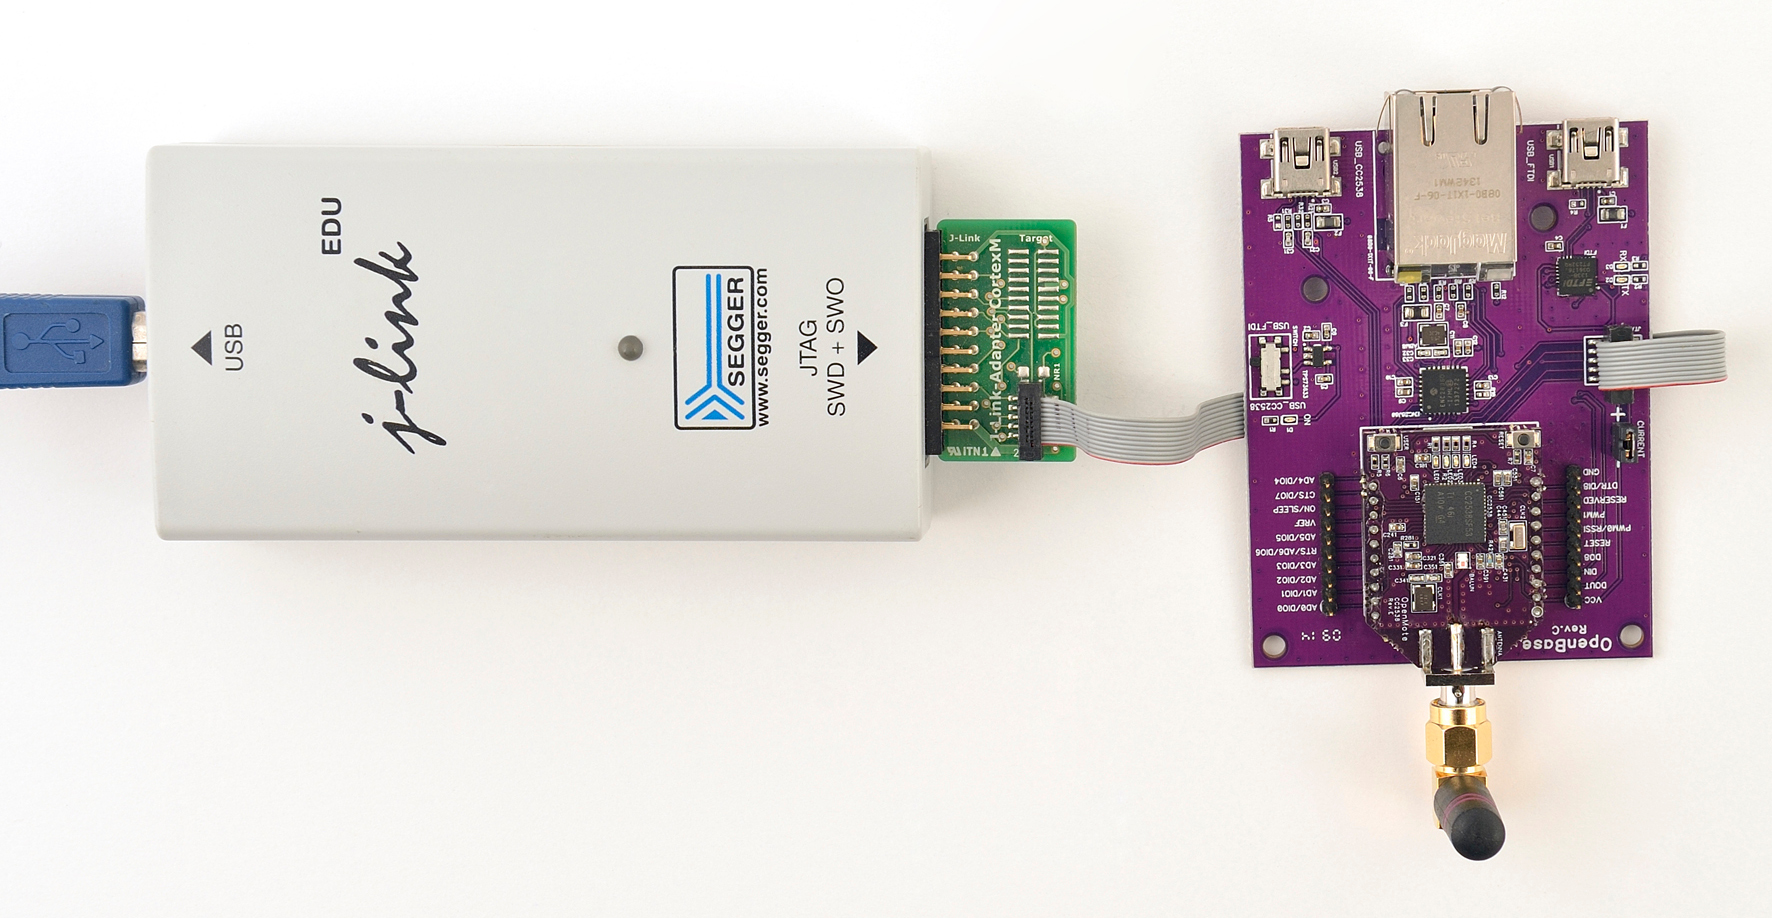
\includegraphics[width=0.75\linewidth]{06-jtag}
    \caption{Connecting the Segger J-Link probe to the OpenBase.}
    \label{fig:06-jtag}
\end{figure}

Once the Segger J-Link is connected to the OpenBase, open another terminal window. This new terminal will execute the Segger J-Link software that allows to connect the JTAG probe with the GDB client that is used to load the code. In the new terminal issue the following commands to go to the appropriate project directory and execute the Segger J-Link software. If connecting the JTAG to the OpenMote-CC2538 is successful, a screen similar to Figure~\ref{fig:06-jlink} should appear.

\begin{verbatim}
cd ~/OpenDQ/projects/Application
make TARGET=cc2538 jlink
\end{verbatim}

% Connecting the JLink to the OpenMote-CC2538
\begin{figure}[!ht]
    \centering
	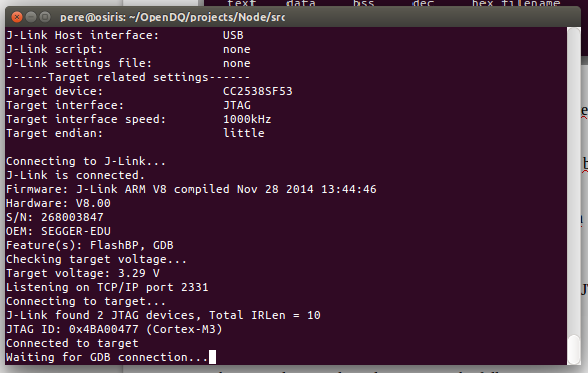
\includegraphics[width=0.75\linewidth]{06-jlink}
    \caption{Connecting the JLink to the OpenMote-CC2538.}
    \label{fig:06-jlink}
\end{figure}

On the original window, execute the following command to load the firmware image to the OpenMote-CC2538. If loading the firmware is successful, a screen similar to Figure~\ref{fig:06-load} should appear. Once the firmware has been loaded, press the reset button on the OpenMote-CC2538 to start executing the code. After that the OpenMote-CC2538 will start blinking the green LED periodically.

\begin{verbatim}
make TARGET=cc2538 load
\end{verbatim}

% Loading the Node/Gateway project with JTAG
\begin{figure}[!ht]
    \centering
	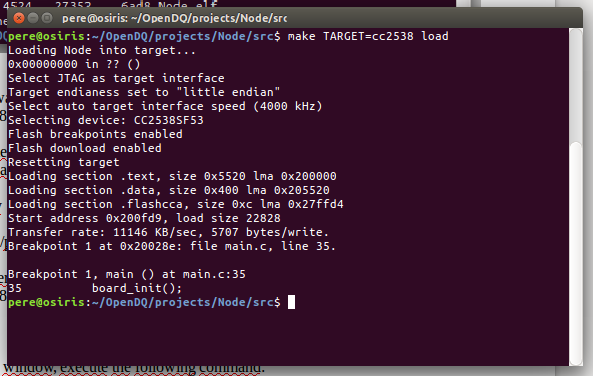
\includegraphics[width=0.75\linewidth]{06-load}
    \caption{Loading the Node/Gateway project with JTAG.}
    \label{fig:06-load}
\end{figure}

In addition to loading the code to the OpenMote-CC2538, with the JTAG mechanism it is also possible to debug execution of the code by either using GDB (command line) or Nemiver (visual interface). In the original terminal window, execute the following commands to start either debugger. If GDB is used a screen similar to Figure~\ref{fig:06-gdb} should appear, whereas if Nemiver is used a screen similar to Figure~\ref{fig:06-nemiver} should appear.

\begin{verbatim}
make TARGET=cc2538 debug
make TARGET=cc2538 nemiver
\end{verbatim}

% Debugging the Node/Gateway project with GDB
\begin{figure}[!ht]
    \centering
	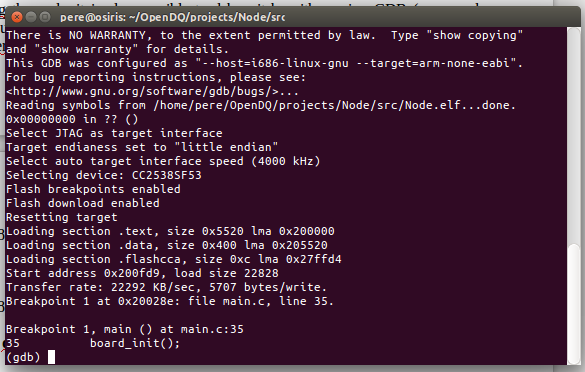
\includegraphics[width=0.75\linewidth]{06-gdb}
    \caption{Debugging the Node/Gateway project with GDB.}
    \label{fig:06-gdb}
\end{figure}

% Debugging the Node/Gateway project with Nemiver.
\begin{figure}[!ht]
    \centering
	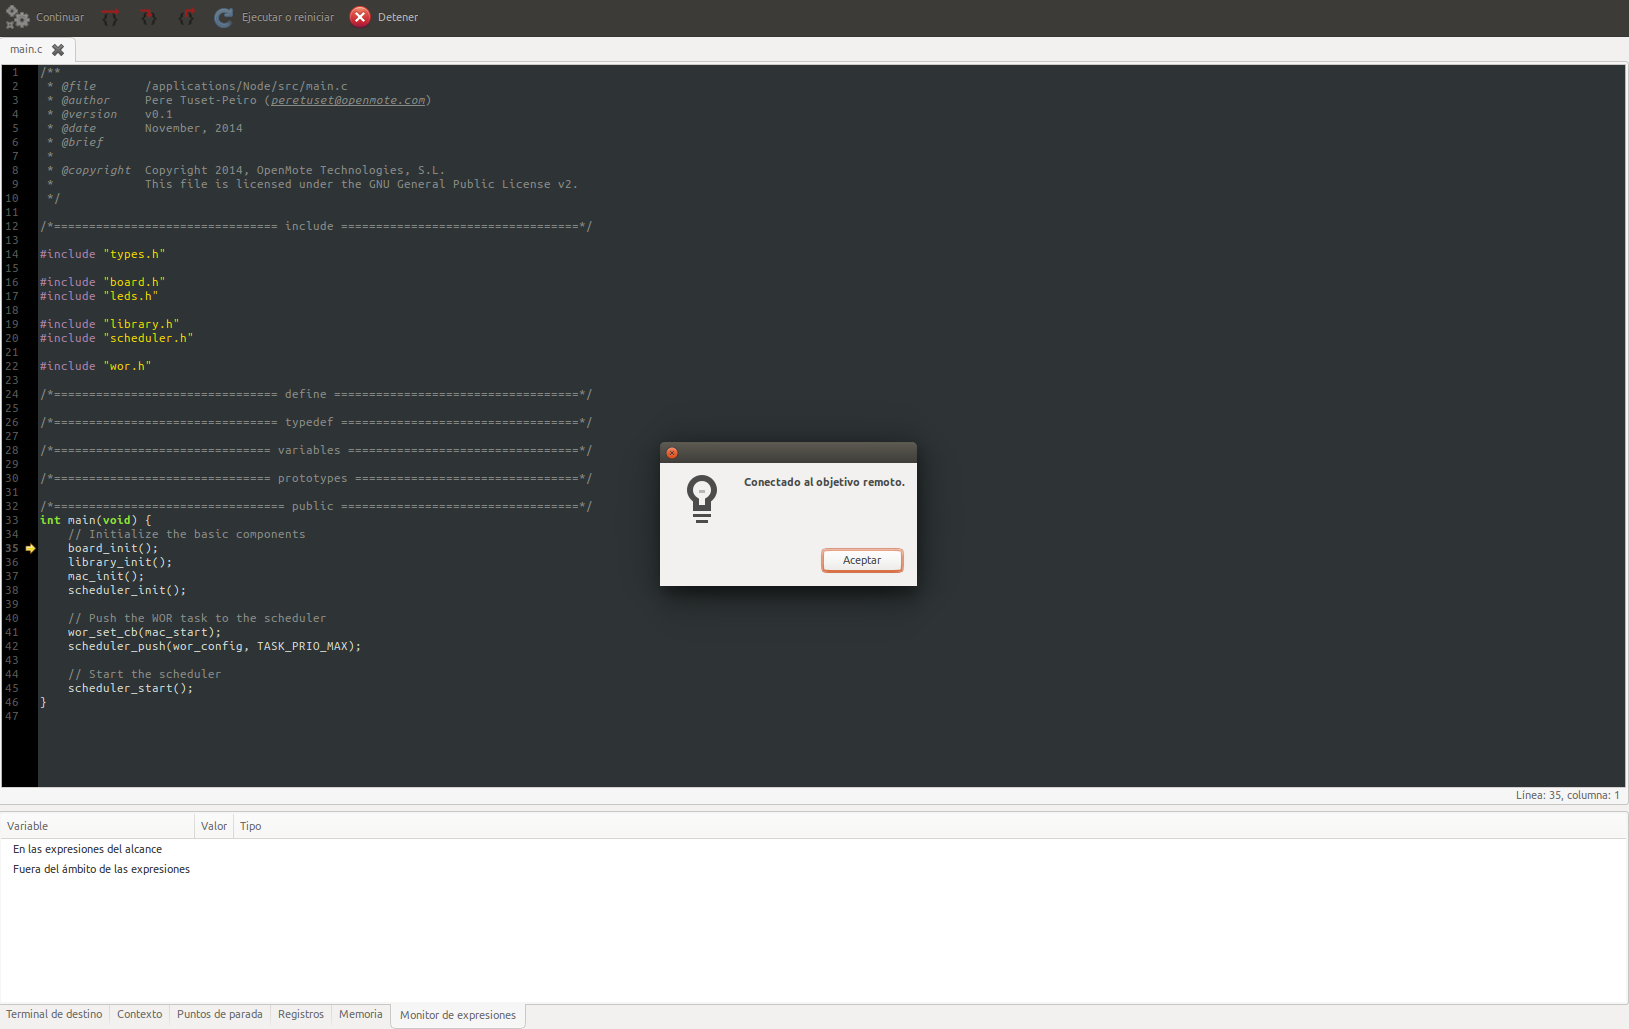
\includegraphics[width=0.75\linewidth]{06-nemiver}
    \caption{Debugging the Node/Gateway project with Nemiver.}
    \label{fig:06-nemiver}
\end{figure}

%%
% Execute the Application projeect
%%
\label{sec:06-software}
\section{Execute the Application project}
To execute the Application project navigate to its directory and start the $OpenDQ\_App.py$ Python script by issuing the following commands. If the command is successfully executed, a screen similar to \ref{fig:06-application} will be displayed.

\begin{verbatim}
cd ~/OpenDQ/projects/Application
python OpenDQ_App.py
\end{verbatim}

% Opening the OpenDQ application
\begin{figure}[!ht]
    \centering
	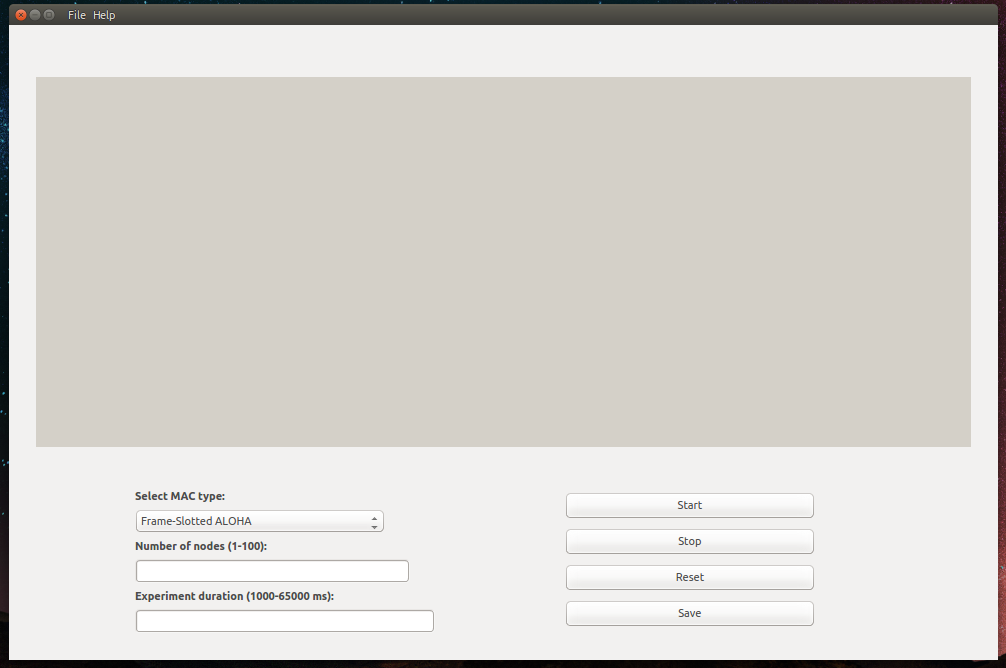
\includegraphics[width=0.75\linewidth]{06-application}
    \caption{Opening the OpenDQ application.}
    \label{fig:06-application}
\end{figure}

The previous command assumes that an OpenMote-CC2538 board is connected to the computer via an OpenBase board using the FTDI port, as depicted in Figure~\ref{fig:06-openbase}. The command also assumes that the Linux kernel is able to detect and load the drivers of the FTDI FT232 chip to create a $/dev/ttyUSBX$ device and that the user has read and write permissions for the given device. If the $/dev/ttyUSBX$ is not detected or the user has no permissions to read and write from the given port the an image similar to Figure~\ref{fig:06-serial_error} will be displayed. If the user has no permissions to read and write from the given port try executing the command with $sudo$ to temporarily gain such permissions.

% Serial port error while opening the OpenDQ application
\begin{figure}[!ht]
    \centering
	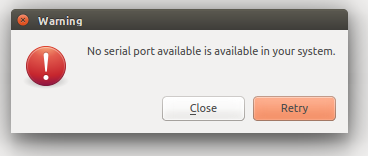
\includegraphics[width=0.75\linewidth]{06-serial_error}
    \caption{Serial port error while opening the OpenDQ application.}
    \label{fig:06-serial_error}
\end{figure}